% 10-16(10쪽) — f(x)=-1/|x+1| 의 그래프(x=-1 을 점근선으로 두 갈래가 아래로). 스캔 화질이 낮아 TikZ 로 다시 그림.
% 원문에 있는 것만: 세로 점선 x=-1 · 라벨 -1, O, x, y, y=f(x).
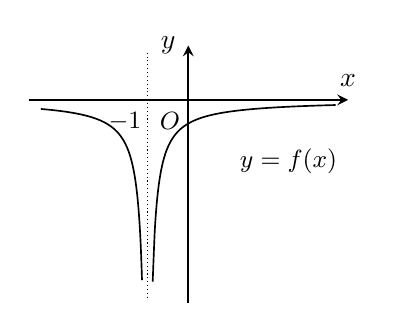
\begin{tikzpicture}[x=0.52cm, y=0.30cm, line width=0.5pt]
  \draw[->, >=stealth, line width=0.7pt] (-3.9,0) -- (3.9,0) node[above=1pt] {$x$};
  \draw[->, >=stealth, line width=0.7pt] (0,-8.6) -- (0,2.3) node[left=1pt] {$y$};
  \draw[densely dotted, line width=0.4pt] (-1,2.0) -- (-1,-8.4);
  \draw[line width=0.6pt, domain=-3.6:-1.13, samples=90, smooth] plot (\x, {-1/(-\x-1)});
  \draw[line width=0.6pt, domain=-0.87:3.6, samples=90, smooth] plot (\x, {-1/(\x+1)});
  \node[below=1pt, font=\small] at (-1.55,0) {$-1$};
  \node[below=1pt, font=\small] at (-0.45,0) {$\pt{O}$};
  \node[right=1pt, font=\small] at (0.95,-2.6) {$y=f(x)$};
\end{tikzpicture}
